\toclesssection{SCP 019 - The Monster Pot}
\addcontentsline{toc}{section}{SCP 019 - The Monster Pot}

\textbf{Item \#:} SCP-019

\textbf{Object Class:} Keter

\begin{figure}[h]
\begin{center}
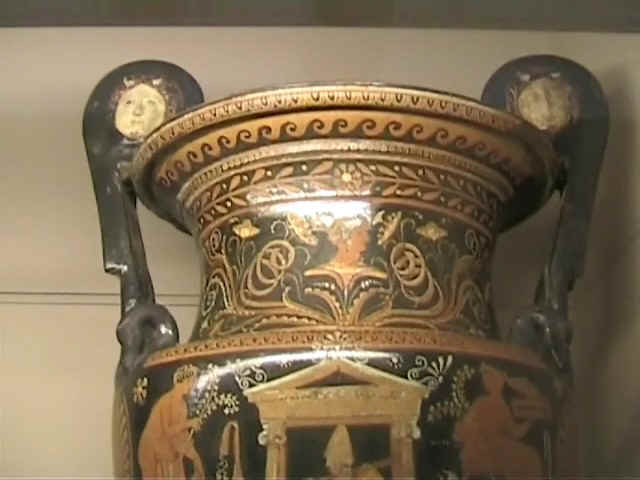
\includegraphics[scale=0.5]{scp/019a.jpg}
\linebreak SCP-019
\end{center}
\end{figure}

\textbf{Special Containment Procedures:} SCP-019 is to be placed on a wide grate in a 3 m x 3 m x 4 m room made of reinforced concrete, installed with an incinerator. Room is to be kept at zero (0) degrees Celsius when incinerator is not activated. An observation chamber separated by a plate glass window is to be used for constant observation of SCP-019, and if/when specimens of SCP-019-2 are noticed, the incinerator is to be activated. In case of an outbreak of SCP-019-2, ordinary firearms are successful in terminating individual specimens, although in the case of a swarm outbreak, flamethrowers may be more effective. SCP-019 should be kept in a vertical position at all times.

\textbf{Description:} SCP-019 appears to be a very large ceramic vase, 1.8 m in diameter at the mouth and 2.4 m high. Style and decoration indicate it was created in Classical Greece, although conclusive dating is impossible, as the surface is entirely unbreakable by any known means. If a successful method is discovered, SCP-019 is to be destroyed with prejudice.

Periodically, entities emerge from SCP-019. Collectively, these are known as SCP-019-2. The entities vary in many aspects, but tend to be small, vaguely humanoid (though they may have animaloid features), and extremely hostile. They often choose to attack with teeth or claws. Although fairly delicate (also, surprisingly, flammable), they are reasonably strong and pose a considerable threat in large numbers.

\begin{figure}[h]
\begin{center}

\includegraphics[scale=0.55]{scp/019b.jpg}
\linebreak SCP-019-2 specimen
\end{center}
\end{figure}

When kept at zero (0) degrees Celsius and totally at rest, entities will emerge from SCP-019 at a rate of approximately one (1) entity per hour. The following traits are known to affect SCP-019-2's manifestation rate:
\begin{itemize}
\renewcommand{\labelitemi}{$\ast$}
\item Movement of SCP-019
\item Threat to SCP-019
\item Extreme temperature in either direction
\item Sudden shift in surrounding environment in general
\item Introduction of objects or organisms to the inside of SCP-019 (known to cause a “flood” reaction)
\end{itemize}
Traits that may or may not influence SCP-019-2's manifestation rate:
\begin{itemize}
\renewcommand{\labelitemi}{$\ast$}
\item Presence of human life near SCP-019
\item Current weather patterns
\item Specific individuals near SCP-019 (some individuals seem to affect SCP-019-2's emergence rate more drastically than others)
\end{itemize}
In addition, tipping or tilting SCP-019 will create a reaction as though it was previously “filled” with SCP-019-2 specimens, although viewers looking into SCP-019 from above will merely note a dark hole. Due to the production rates of SCP-019-2 when the object is disturbed, measurement of the internal cavity is difficult, but it is suspected to be inconsistent with outside measurements.

\textbf{Addendum:} Document SCP-019-2-A
SCP-019-2 notes, as maintained by Doctor Light and Doctor Vaux

\censor{XX}/\censor{XX}/\censor{XXXX}\linebreak
SCP-019-2 specimen was removed from containment chamber and kept in reinforced pen, provided with water and live chickens as food. Specimen made quiet, continuous, garbled vocalizations, determined to be phonetically similar to Ancient Hellenic languages. Although it is unknown why this is, specimens are still thought to be no more intelligent than animals.

The specimen only lived for under 48 hours, and a dissection revealed anatomy consistent on a cellular level with normal biology, but with an extremely unstable musculoskeletal structure. Other notable anomalies included an unstable respiratory system, next to no digestive tract, and virtually no other internal organs. All other captured specimens have followed similar patterns of behavior and demise.

Note: It appears that SCP-019-2 specimens were not intended to live for meaningful amounts of time outside of SCP-019. - Dr. Vaux

\censor{XX}/\censor{XX}/\censor{XXXX}\linebreak
Containment unit was slightly damaged following prolonged exposure to SCP-019-2 specimen, missed by the monitoring team because of partial transparency. This has not been noted in SCP-019-2 before. Monitoring teams will continue to report further anomalies.

\censor{XX}/\censor{XX}/\censor{XXXX}\linebreak
Monitoring teams report some specimens of SCP-019-2 now appear to be significantly more resistant to incineration than others. It is hypothesized that this is a defense mechanism on the part of SCP-019.

\censor{XX}/\censor{XX}/\censor{XXXX}\linebreak
Most specimens of SCP-019-2 are now all but entirely resistant to the effects of the incinerator. Use of acid bath instead of incinerator is being considered. “Evolution” of SCP-019-2 is being studied, and may be evidence of sentience in SCP-019-2.